\chapter{Aufbau Projekt}
Im folgenden wird anhand der verschiedener Bereiche die Funktionsweise des Programmes erläutert. 


\section{Projektstruktur}
\subsection{Projekt kickstarten}
Zu Beginn der Entwicklung war es nötig, eine Basis für die Anwendung zu haben. Zu dieser Basis gehörten
\begin{itemize}
\item \textbf{GitHub Repository} zur Versionsverwaltung des Codes
\item \textbf{Konfigurations-Einstellungen in package.json} zur Verwaltung der von nodeJS benötigten Pakete
\item \textbf{Konfigurations-Einstellungen in bower.json} zur Verwaltung der Pakete des FrontEnds
\item \textbf{Grundfile.js} mit allen Tasks, die während der Entwicklung und zum Deployment zum Einsatz kommen
\item \textbf{Ordner-Struktur} für Module und die eigentliche Anwendung
\end{itemize}

Dies per Hand zu machen, ist generell sehr fehleranfällig und benötigt einige Zeit. Aus diesen Gründen wurde hierbei die NodeJS-Kickstarter-Anwendung \textit{yeoman.io} verwendet.
Diese Anwendung stellt verschiedene Generatoren zur Verfügung, mit welchen sich unterschiedlichste Anwendungen kickstarten lassen. Aktuell umfasst die Generatoren-Bilbliothek mehr als 4800 verschiedene
Generator-Module.\\
Die vorliegende Anwendung wurde mithilfe des Generators "angular" gekickstartet. "angular" ist ein offizielles vom Yeoman-Team entwickeltes Modul.
Über den Konsolenbefehl\\
\texttt{yo generator:angular App}\\
generiert Yeoman alle oben genannten Strukturen, Dateien der Boilerplate-Angular-Anwendung und Test-Methoden.
Da es sich bei AngularJS-Anwendungen meistens um Single-Page-Anwendungen handelt, ist die Ausgangdatei die \textit{index.html}-Datei im App-Ordner.
In dieser Datei werden alle Javascript-Module und CSS-Bibliothenek zusammengeführt. Dabei zeichnet sich ein großer Vorteil von der Verwendung von Yeoman heraus:
In der HTML-Datei befinden sich Marker, mit welchen die Bereiche markiert sind, in denen Javascripte und Stylesheets eingebaut werden. Installiert ein Benutzer über Bower neue Module, so erfolgt das Einbinden automatisch.
Gesteuert wird dieser Prozess von dem \texttt{serve}-Task in \textit{Gruntfile.js}.\\
Eine weitere sehr nützliche Funktion, ist die Möglichkeit, neue AngularJS-Module, wie z.B. Controller, Services oder Direktiven direkt über die Kommandozeile hinzuzufügen.
Die Erstellung des Kontrollers erfolgt über den Befehl \\
\texttt{yo angular:controller ControllerName}\\
Über diesen Befehl generiert Yeoman nun einen Angular-Controller, der in dem entsprechenden controller-Ordner abgelegt wird. Dieser Controller ist bereits mit der existierenden Anwendung
 verknüpft. Zudem wird das JS-File direkt in die \textit{index.html}-Datei eingebunden.\\
 Zusammengefasst erleichtert es die Verwendung eines Generators, wie in diesem Falle Yeoman, Grundlagen für eine Anwendung zu schaffen und diese in ihrer Entwicklung vornzutreiben.
\subsection{grunt serve}

%TODO write something about the structur and kickstart and so on

\section{Frontend}
Der für den Nutzer sichtbare Bereich.
\subsection{Login}
Da die Software wie bereits erwähnt nicht nur intern im Büro sondern auch von extern aus erreichbar sein muss, ist es nötig eine Authentifizierung einzurichten damit unbefugte keine Möglichkeiten haben die Daten zu verändern. Um die Software nutzen zu können, benötigt der Bearbeiter eine gültige Kombination aus E-Mail und Passwort. Schon bei der Eingabe der Daten wird überprüft, ob die Felder leer sind oder es sich dabei um eine E-Mail handelt oder nicht. Dabei wird darauf hingewiesen sobald das AT -Zeichen oder der Punkt fehlt. 

Sobald das Formular abgeschickt wurde, werden die Daten zunächst im \texttt{login.js} Controller entgegengenommen. Von da aus werden die Daten an Authenticate-Service weitergegeben. Dort werden diesen an das Backend geschickt. In Firebase werden diese dann mit den hinterlegten Daten verglichen. Sind die Angaben nicht korrekt wird eine Fehlermeldung zurückgegeben die der Controller im View anzeigt. Sofern alles richtig ist, wird der Nutzer weiter zu der Hauptseite geleitet. 

Da es sich hierbei um eine Betriebsinterne Software handelt wird eine Registrierung nicht benötigt. Die Emailadresse und das Passwort werden Manuell im Backend hinzugefügt, bearbeitet oder entfernt. 

\begin{figure}[H]
\centering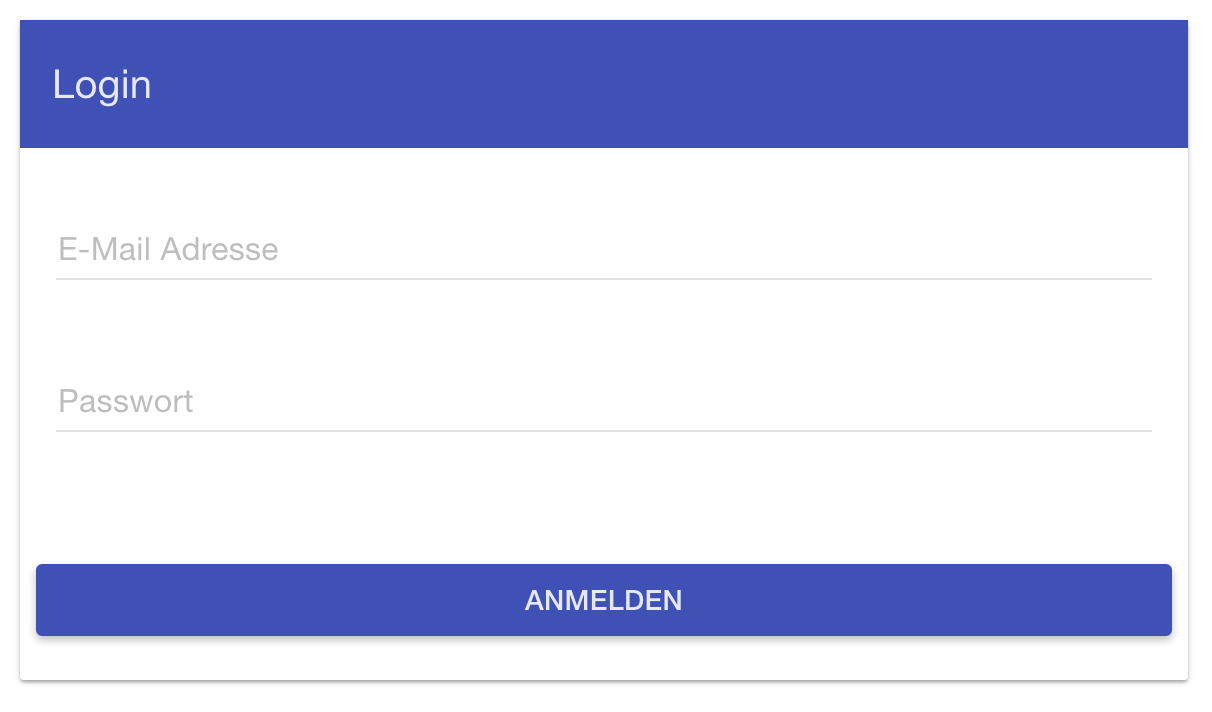
\includegraphics[width=0.5\textwidth]{images/frontend_login.png}
\caption{Frontend \texttt{Login}}
\label{Login}
\end{figure}

\subsection{Hauptseite}
Die Hauptseite ist sehr schlicht aufgebaut und teilt sich auf in zwei Teile. 

\begin{figure}[H]
\centering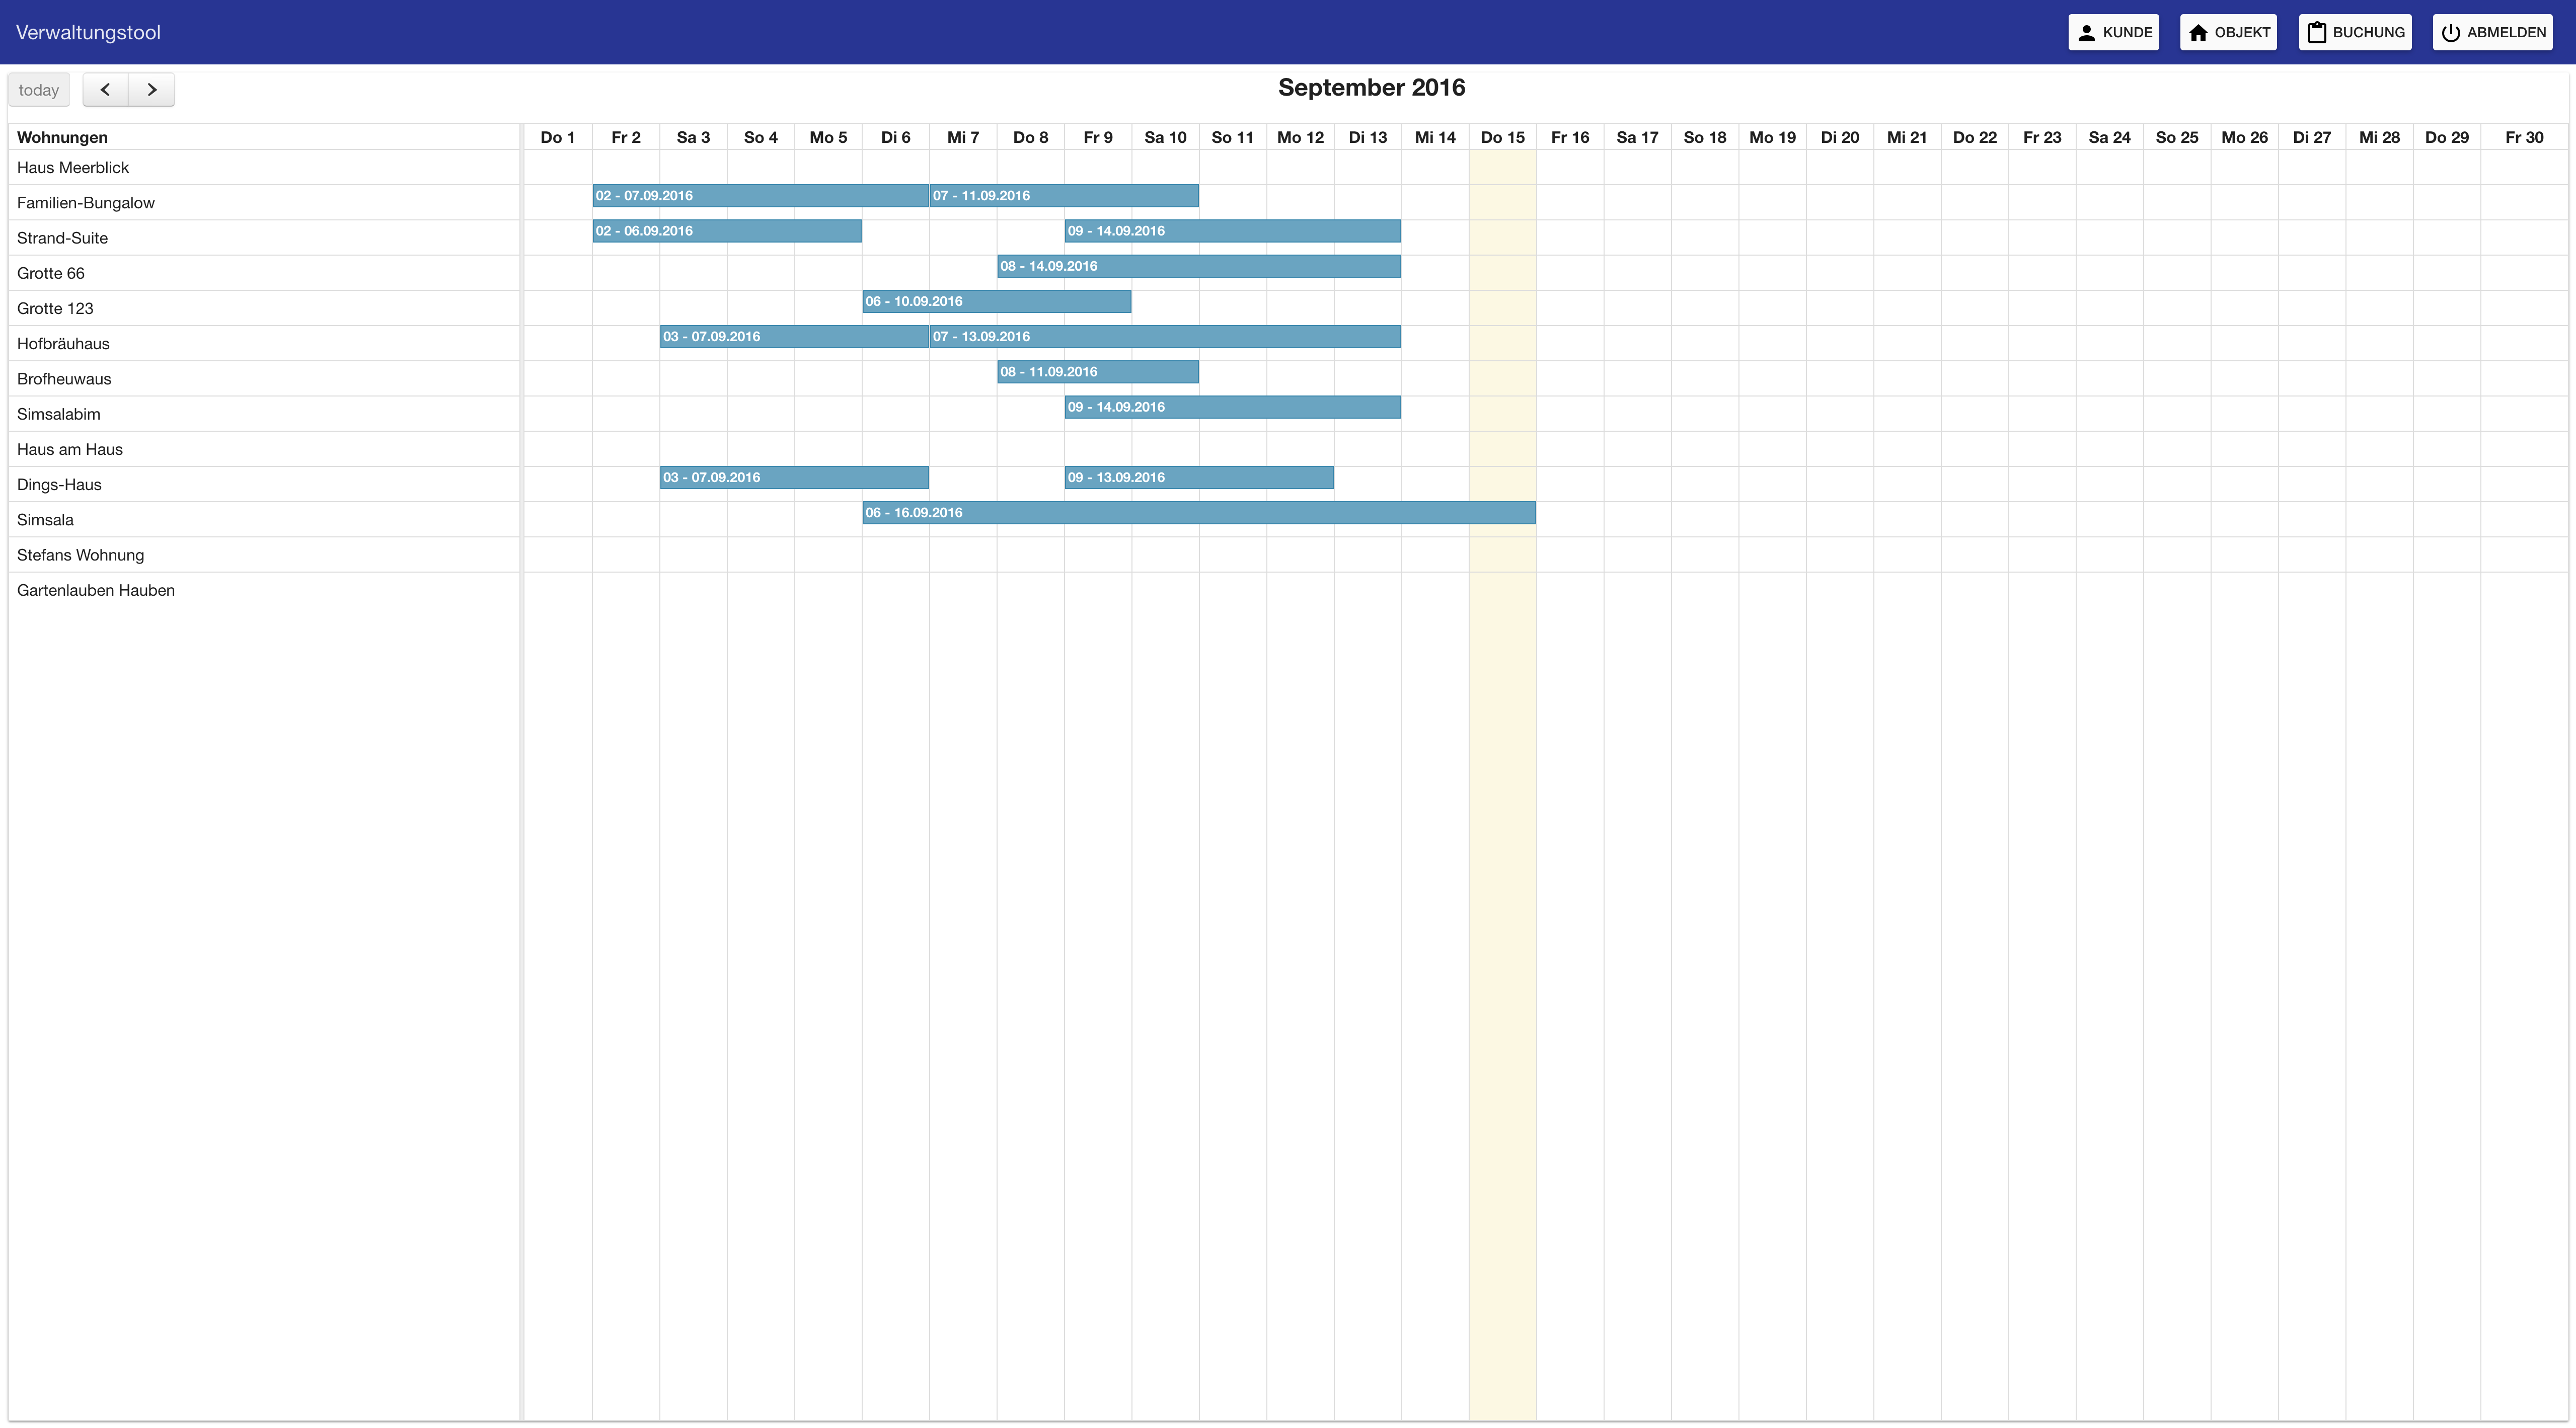
\includegraphics[width=1\textwidth]{images/frontend_mainpage.png}
\caption{Frontend \texttt{Hauptseite}}
\label{Hauptseite}
\end{figure}

\subsubsection{Header}
Im Header befinden sich neben dem Programmlogo auch folgende vier Button:


\begin{minipage}{0.6\textwidth}
\begin{description}
\item[Kunde]\hfill \\
Ein Dialog öffnet sich in dem Kunden hinzugefügt, bearbeitet oder gelöscht werden können.
\item[Objekt]\hfill \\ 
Ein Dialog öffnet sich in dem eine neue Ferienwohnung / Haus hinzugefügt werden kann. 
\item[Buchung]\hfill \\ 
Ein Dialog öffnet sich in dem eine neue Buchung hinzugefügt werden kann. 
\item[Logout]\hfill \\ 
Nach der Bestätigung eines Dialogs wird der Nutzer abgemeldet und auf die Login-Seite verwiesen. 
\end{description}

Sobald die Fenstergröße kleiner oder die Größe eines durchschnittlichen Tablets erreicht hat, werden die Buttons ausgeblendet. Stattdessen erscheint ein Symbol das bei Klick eine Seitennavigation einblendet in der sich alle Buttons befinden.
\end{minipage}
\hspace{0.05\textwidth}
\begin{minipage}{0.35\textwidth}
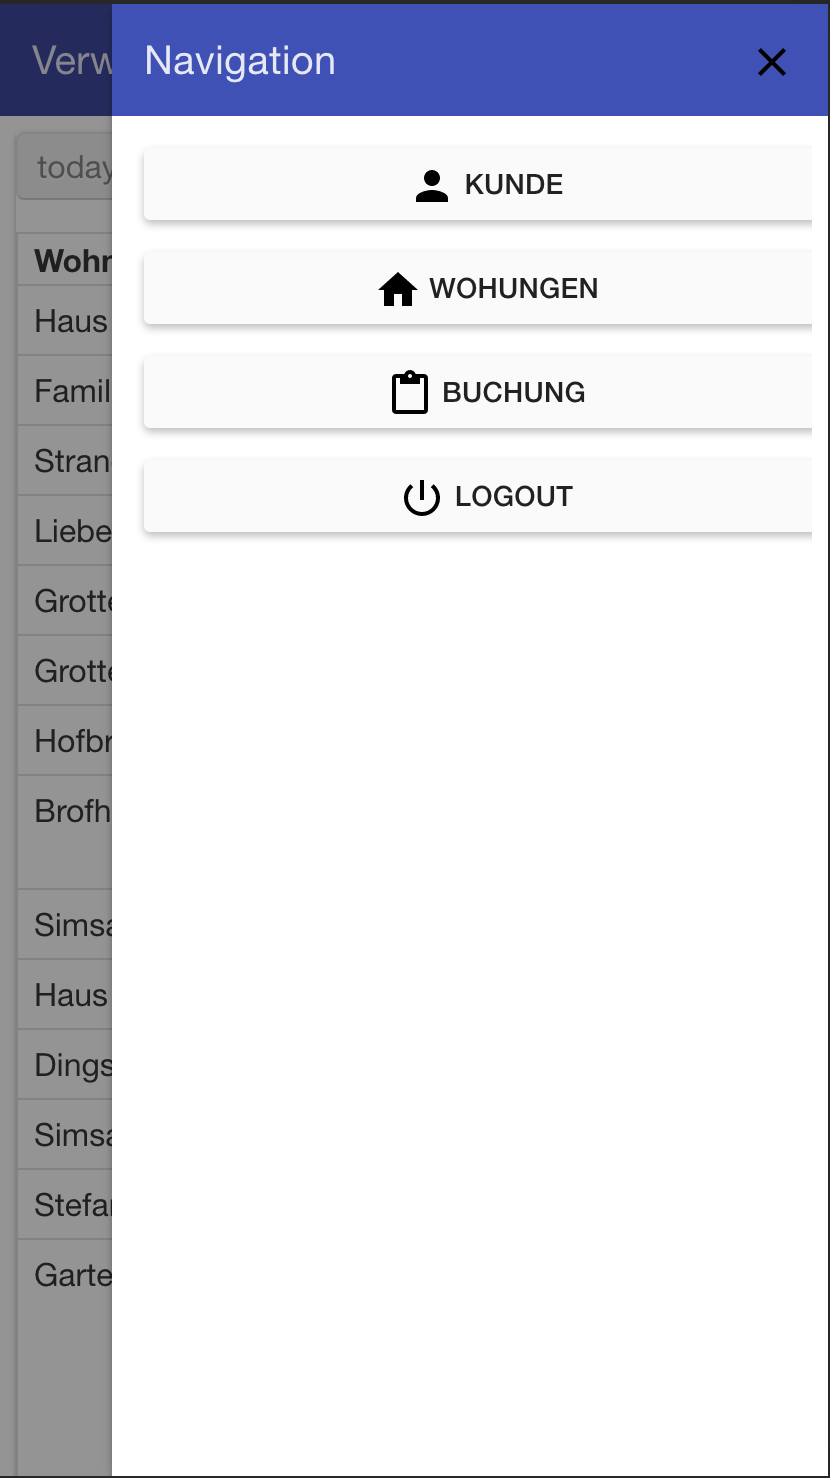
\includegraphics[width=\textwidth]{images/frontend_header_small.png}
\end{minipage}





\subsubsection{Main}
In der Main befindet sich lediglich der Kalender, welcher auf voller Breite und Höhe abgebildet. 
Dieser ist aufgeteilt in folgende zwei Bereiche:
\begin{description}
\item[Objektübersicht]\hfill \\
Alle Objekte werden auf der linken Seite in form einer Liste dargestellt
\item[Buchungsübersicht]\hfill \\ 
Alle Tage des aktuellen Monats werden als Spalten angezeigt. Die Buchungen werden als Blöcke angezeigt und verbinden dessen Tage in Spalten.  
\end{description}

\subsection{Kunde}
Zusammen mit dem Objekt bildet der Kunde eine Buchung. Für die Kundeninformationen wurden alle Felder aus dem Projektzielen implementiert. Zudem sind alle Felder ausgenommen der Zusatzinformationen und der Firma Pflicht und werden beim Abschicken des Formulars überprüft, ob sie leer sind. Um die Eingabe des Geburtstages zu vereinfachen wurde ein für Tag, Monat und Jahr jeweils ein Dropdown-Menü bereitgestellt. Da das Mindestalter für Buchungen 18 Jahre ist, ist das höchste auszuwählende Jahr immer 18 Jahre vom aktuellen gerechnet. Das Datum wird im UNIX TIMESTAMP gespeichert. Sind alle Felder korrekt ausgefüllt, kann das Formular abgeschickt werden. Sobald die \texttt{submit} Funktion im Controller aufgerufen wird, werden alle Felder aus dem View einem \texttt{customer} JSON-Objekt gespeichert. Diese werden dem \texttt{Customer} Model übergeben und das Dialog geschlossen. 

Soll ein bestehender Kunde bearbeitet werden muss dieser zunächst über das Suchfeld gesucht werden. Mittels des Lupensymbol im Kopfbereich des Dialog wird die Suchleiste ein oder ausgeblendet. Sobald das Suchfeld fokussiert wird, wird eine Funktion im Controller angestoßen welche alle Kunden mit Vor und Nachname als Auswahlmöglichkeit auflistet. Dafür wird die Liste aller Kunden im Model angefordert. Dieses Liefert ein Array mit allen Kundenobjekten. Bei einer hohen Anzahl an Kunden kann sich die Suche schwierig gestalten. Aus diesem Grund kann der Kunde durch eintippen von Buchstaben gefiltert werden. Jeder weitere Buchstabe schränkt die Suche nach dem Vornamen ein und es werden nur Kunden angezeigt dessen Vornamen die eingegebene Zeichenkette beinhalten. 

Wurde ein Kunde ausgewählt, werden alle Daten aus dem JSON-Objekt ausgelesen und in die Input Felder eingefügt. Gleichzeitig wird ein Button angezeigt der das Löschen eines Kunden aus der Datenbank ermöglicht. Um einem Fehler vorzubeugen muss zusätzlich noch ein Dialog bestätigt werden. Wird dieser bestätigt übergibt der Controller dem Model die UUID des Kunden in einer \texttt{delete} Funktion. 
%TODO delete customer in model

Wenn Daten verändert wurden, können diese wie auch beim Hinzufügen eines neuen Kunden bestätigt werden. Dabei wird die selbe Funktion aufgerufen. In diesem Fall wird im Controller die \texttt{upsert} Funktion im Model aufgerufen. Je nachdem, ob es sich dabei um einen bestehenden Eintrag in der Datenbank handelt oder der Eintrag bereits vorhanden ist wird ein \texttt{Update} oder \texttt{Insert} durchgeführt. Dafür ist die von der Datenbank vergebene UUID ausschlaggebend.

Soll weder ein neuer Kunde hinzugefügt noch ein bestehender bearbeitet werden kann das Dialog über den \grqq Abbrechen\glqq Button, das \grqq X\glqq oder einen Klick ausserhalb des Dialogs geschlossen werden. Für den Controller ist das ein und die selbe Funktion. Dieser ruft lediglich die \texttt{hide} Methode des Dialogs auf und das Dialogfenster wird ausgeblendet. Dabei werden auch alle Daten aus den Feldern entfernt.

\begin{figure}[H]
    \centering
    \begin{minipage}[t]{0.49\linewidth}
        \centering
        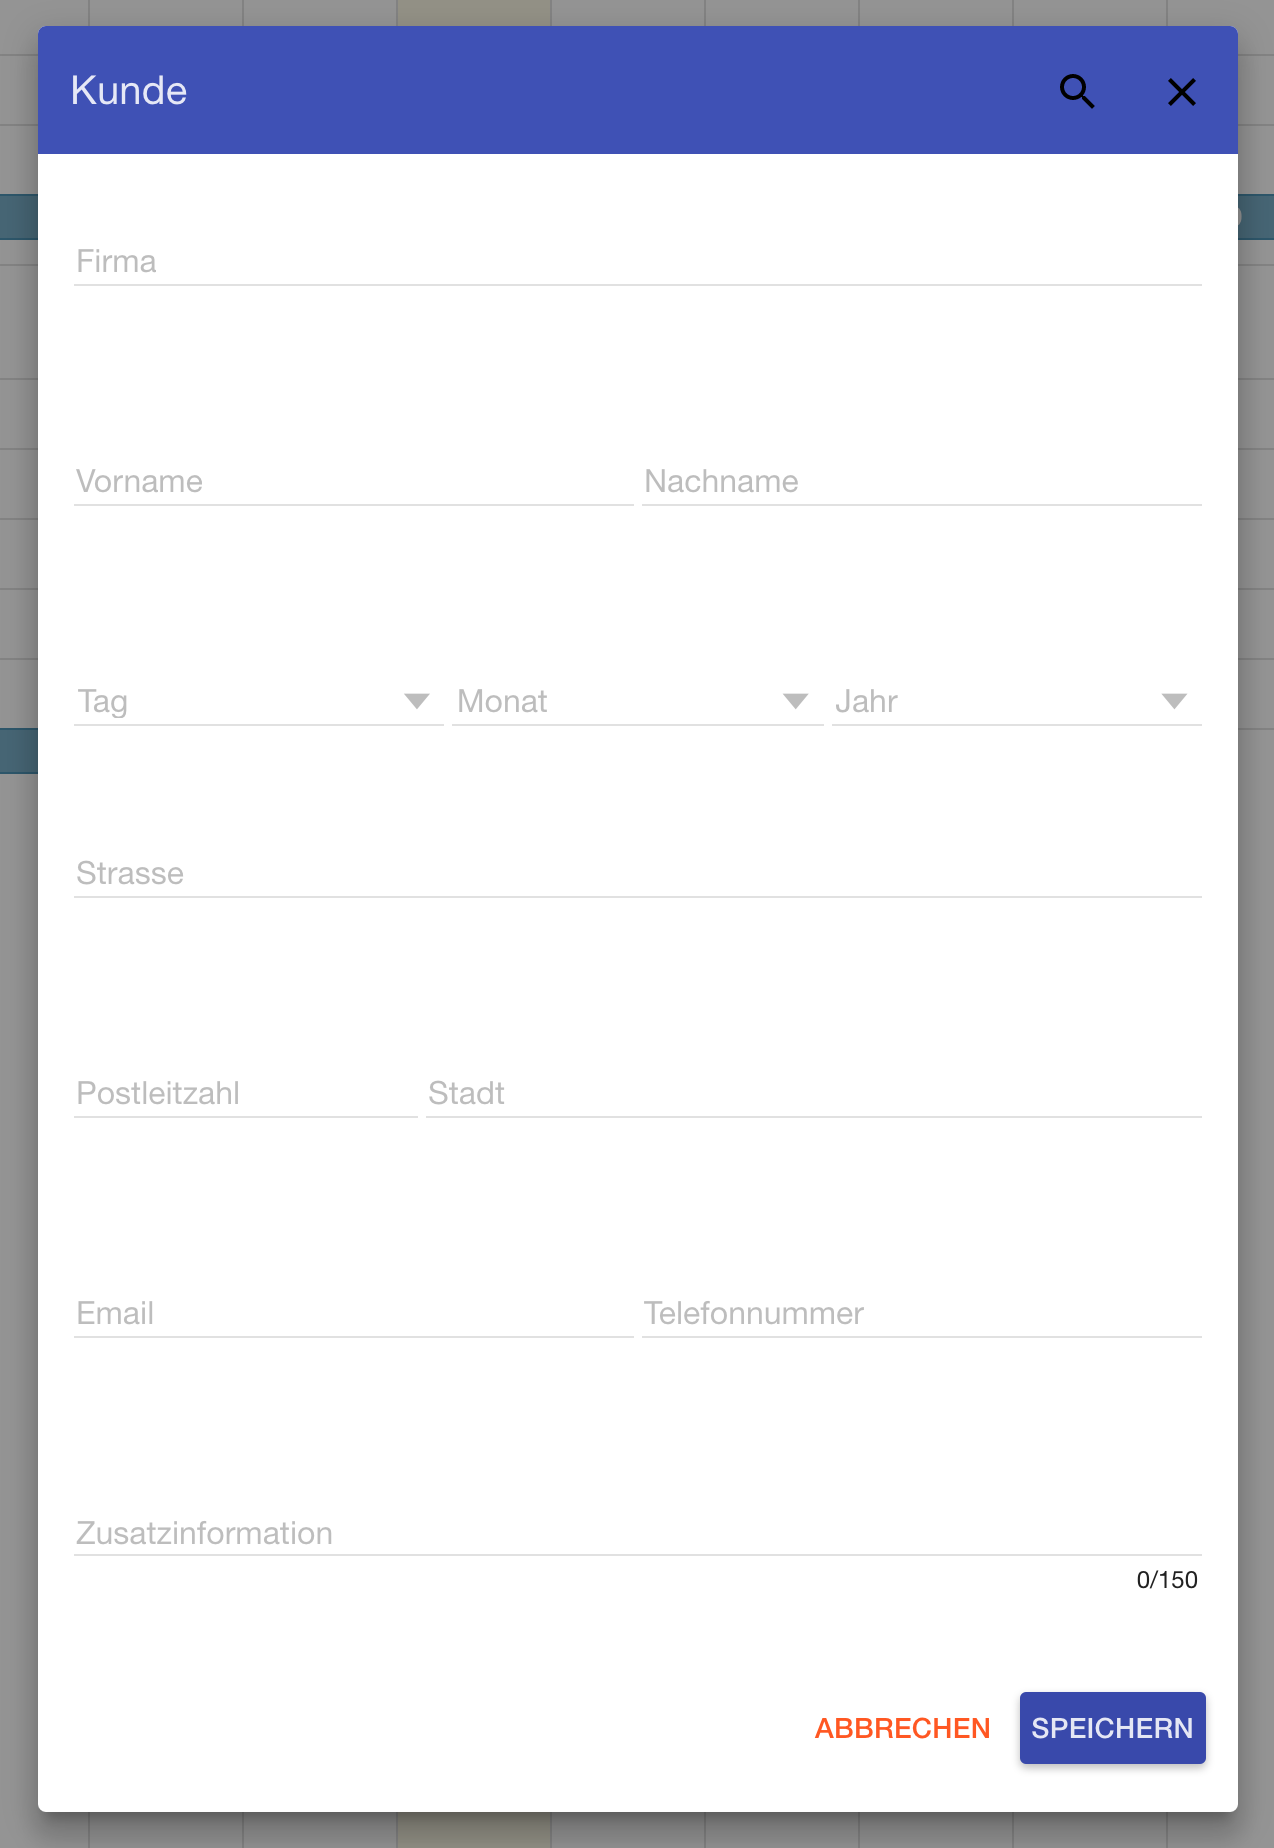
\includegraphics[width=\linewidth]{images/frontend_customer_new.png}
        \caption{Neuen Kunden erstellen}
    \end{minipage}% <- sonst wird hier ein Leerzeichen eingefügt
    \hfill
    \begin{minipage}[t]{0.49\linewidth}
        \centering
        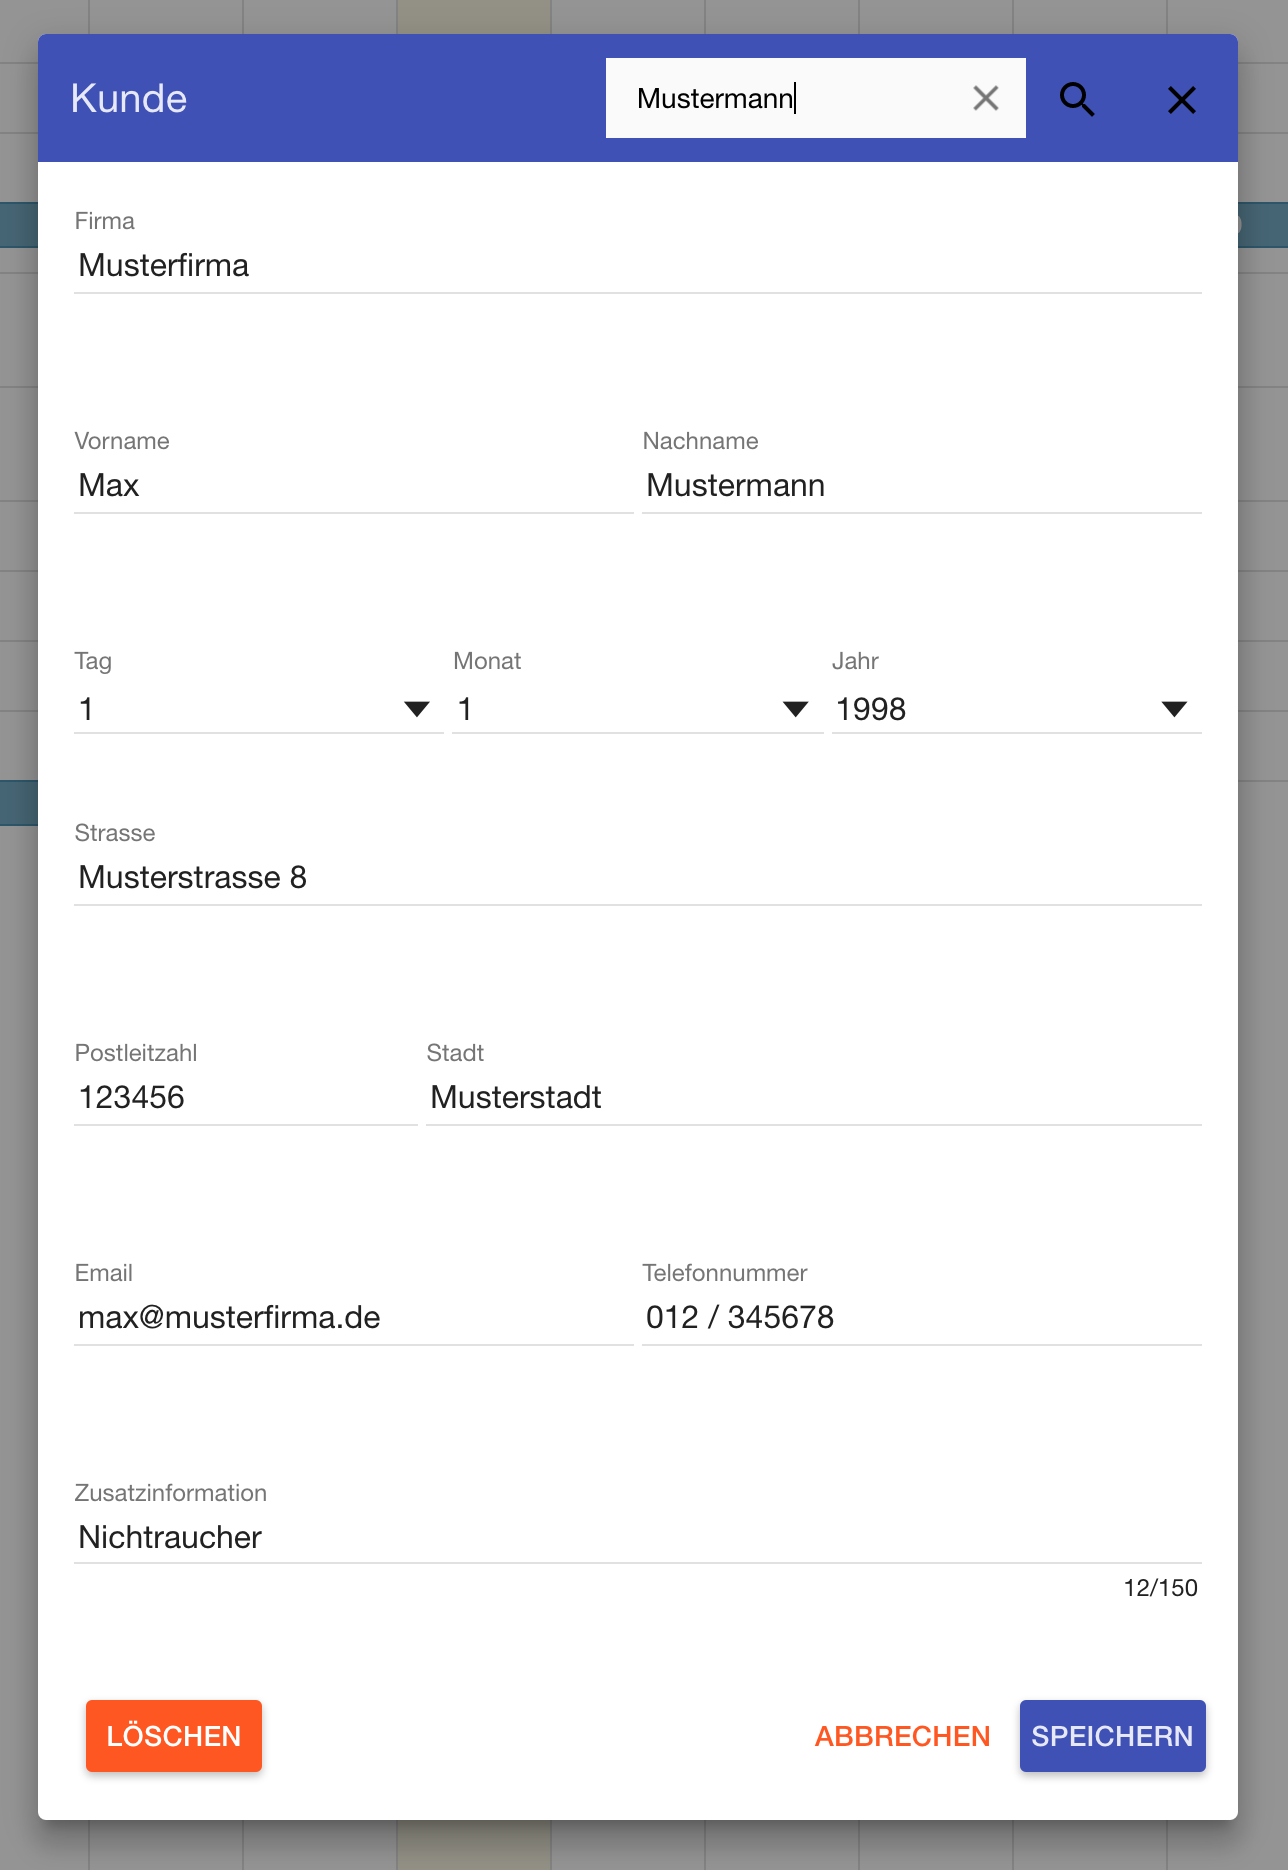
\includegraphics[width=\linewidth]{images/frontend_customer_edit.png}
        \caption{Kunden bearbeiten}
    \end{minipage}
\end{figure}



\subsection{Objekt}
Als Objekt wird eine Ferienwohnung oder Haus bezeichnet. Wie auch beim Kunden können Objekte verschiedene Informationen gespeichert werden. Die beiden gewünschten Felder aus den Projektzielen wurden übernommen. Dazu gehört die Eingabe des Namens in ein Textfeld. Wird das Feld fokussiert und ohne Eingabe verlassen erscheint eine Fehlermeldung mit dem Hinweis das Feld auszufüllen. Wird dieser Hinweis ignoriert und der Nutzer versucht das Formular abzuschicken, überprüft der View, ob alle als Pflicht gekennzeichneten Felder ausgefüllt wurden und der \texttt{submit} Button gedrückt wurde. Ist eines dieser Angaben \texttt{false} wird das Formular erst gar nicht abgeschickt. Auch bei der Angabe der maximalen Personenanzahl wurde darauf geachtet Falscheingaben abzufangen. Standardmäßig ist das minimum von 1 eingestellt. Der Nutzer hat die Möglichkeit mit Hilfe von Pfeilen den Wert zu Verändern. Die Maximale Anzahl von Personen ist 10 für jedes Objekt. Da es auch möglich ist Manuell eine Zahl einzugeben, wird ebenfalls überprüft, ob sich die Zahl in der Range zwischen 1 und 10 befindet. Ist dies nicht der Fall wird ein Hinweis ausgegeben und das Formular kann nicht abgeschickt werden. Sind alle Angaben korrekt und der \texttt{submit} Button wird betätigt wird das Formular abgeschickt. Im Controller wird eine Funktion aufgerufen in der die Daten aus den Feldern in ein JSON-Objekt gespeichert werden. Dieses wird der \texttt{upsert} Methode des Models übergeben. 

Um ein bereits existierendes Objekt bearbeiten zu können muss dies anders als bei den Kunden in der Auflistung in der main ausgewählt werden. Auch hier werden die Daten anhand der UUID aus der Datenbank geladen und in die Felder eingefügt. Zusätzlich wird der Button zum Löschen des Objektes angezeigt. Die Besonderheit bei der Änderung von Daten ist eine Eigenschaft im JSON-Objekt in dem die Informationen der Felder gespeichert werden. Neben des Namens und der Personenanzahl wird die ID des Objektes gespeichert. Ist, wie bei einer Änderung, bereits eine UUID vorhanden, wird diese als Wert gespeichert. Wird eine Objekt neu hinzugefügt ist der Wert \texttt{undefined}. Diese Information erlaubt wird in der \texttt{upsert} Methode des Models abgefragt und dementsprechend ein neues Objekt hinzugefügt oder ein bestehendes aktualisiert.
%TODO how works upsert at model

  
\subsection{Buchung}
Eine Buchung ist ein Zusammenschluss aus Kunde, Objekt, Personenanzahl, Startdatum und Enddatum. Wie bei der Bearbeitung von Kunden, kann der Nutzer den Kunden über ein Suchfeld filtern und Auswählen. Zusätzlich funktioniert das ebenfalls für das Objekt. 
%TODO load data from model
Wenn eine neue Buchung hinzugefügt wird, wird zunächst die Auswahl der Personenanzahl ausgeblendet. Erst wenn ein Objekt im Suchfeld ausgewählt wurde, wird die Auswahl in form eines Dropdown-Menüs im View angezeigt. Im Controller wird vorher die maximale Personenanzahl des ausgewählten Objektes aus dem JSON-Objekt entnommen und somit die zur Auswahl stehenden Zahlen ermittelt. So zeigt das Dropdown-Menü nur genau die Anzahl von Personen an die dieses Objekt zur verfügung stellt. Für das Startdatum und Enddatum wurden, anders als beim Kunden, ein Datepicker zur verfügung gestellt, der es dem Nutzer erlaubt das Datum durch einfache Auswahl in einem Kalender festzulegen. Standardmäßig ist das aktuelle Datum eingestellt.

Um eine Buchung bearbeiten zu können muss diese anders als beim Kunden oder Objekt zunächst in der Buchungsübersicht gesucht werden. Wurde die passende Buchung gefunden und ausgewählt, öffnet sich das Modal mit den hinterlegten Daten. Hier wird die Personenauswahl angezeigt und mit dem eingetragenem Wert vordefiniert. Auch hier besteht die Möglichkeit durch den angezeigten Löschen-Button die Buchung aus der Datenbank zu entfernen.  

Wird ein Dialog bestätigt wird erscheint für drei Sekunden am oberen rechten Fensterrand ein Nachricht. Ein sogenannter Toast fährt herunter und zeigt die Erfolgsmeldung und einen Button zum schließen an. In der mobilen Ansicht fährt der Dialog, in voller Bildschirmbreite, von unten herein. 

\subsection{Kalender}

%TODO write text about the main calender
 
\section{Backend}
